\section{Realisering og test}
\label{realiseringOgTest}

%Her kan du skrive om realisering og test

Figur \ref{fig:Fig2} viser den realiserte løsningen på et overordnet nivå. Telleren som er nevnt i den prinsipielle løsningen er realisert med en adderer som tar inn binære 3-bits tall fra d-vippene i slutten av kretsen og legger det sammen med et fast binært tall. Deretter går signalet inn i en 3-bit mux med to innganger, som vil resete kretsen til 001 dersom signalet blir 110. D-vippene lagrer dataen og sender det nåværende tallet tilbake til addereren og starter kretsen på nytt. Med denne oppkoblingen er det klokken til d-vippen som bestemmer hvor raskt telleren teller. Deretter er det et register med d-vipper som lagrer verdien til telleren ved en stigenede flanke og på den måten lagre et tilfeldig tall fra telleren og sende det videre til dekoderen.Dekoderen tar inn et 3-bit signal og bestemmer hvilke LEDs i matrisen som skal lyse.

\begin{figure}[htbp]
  \centering
  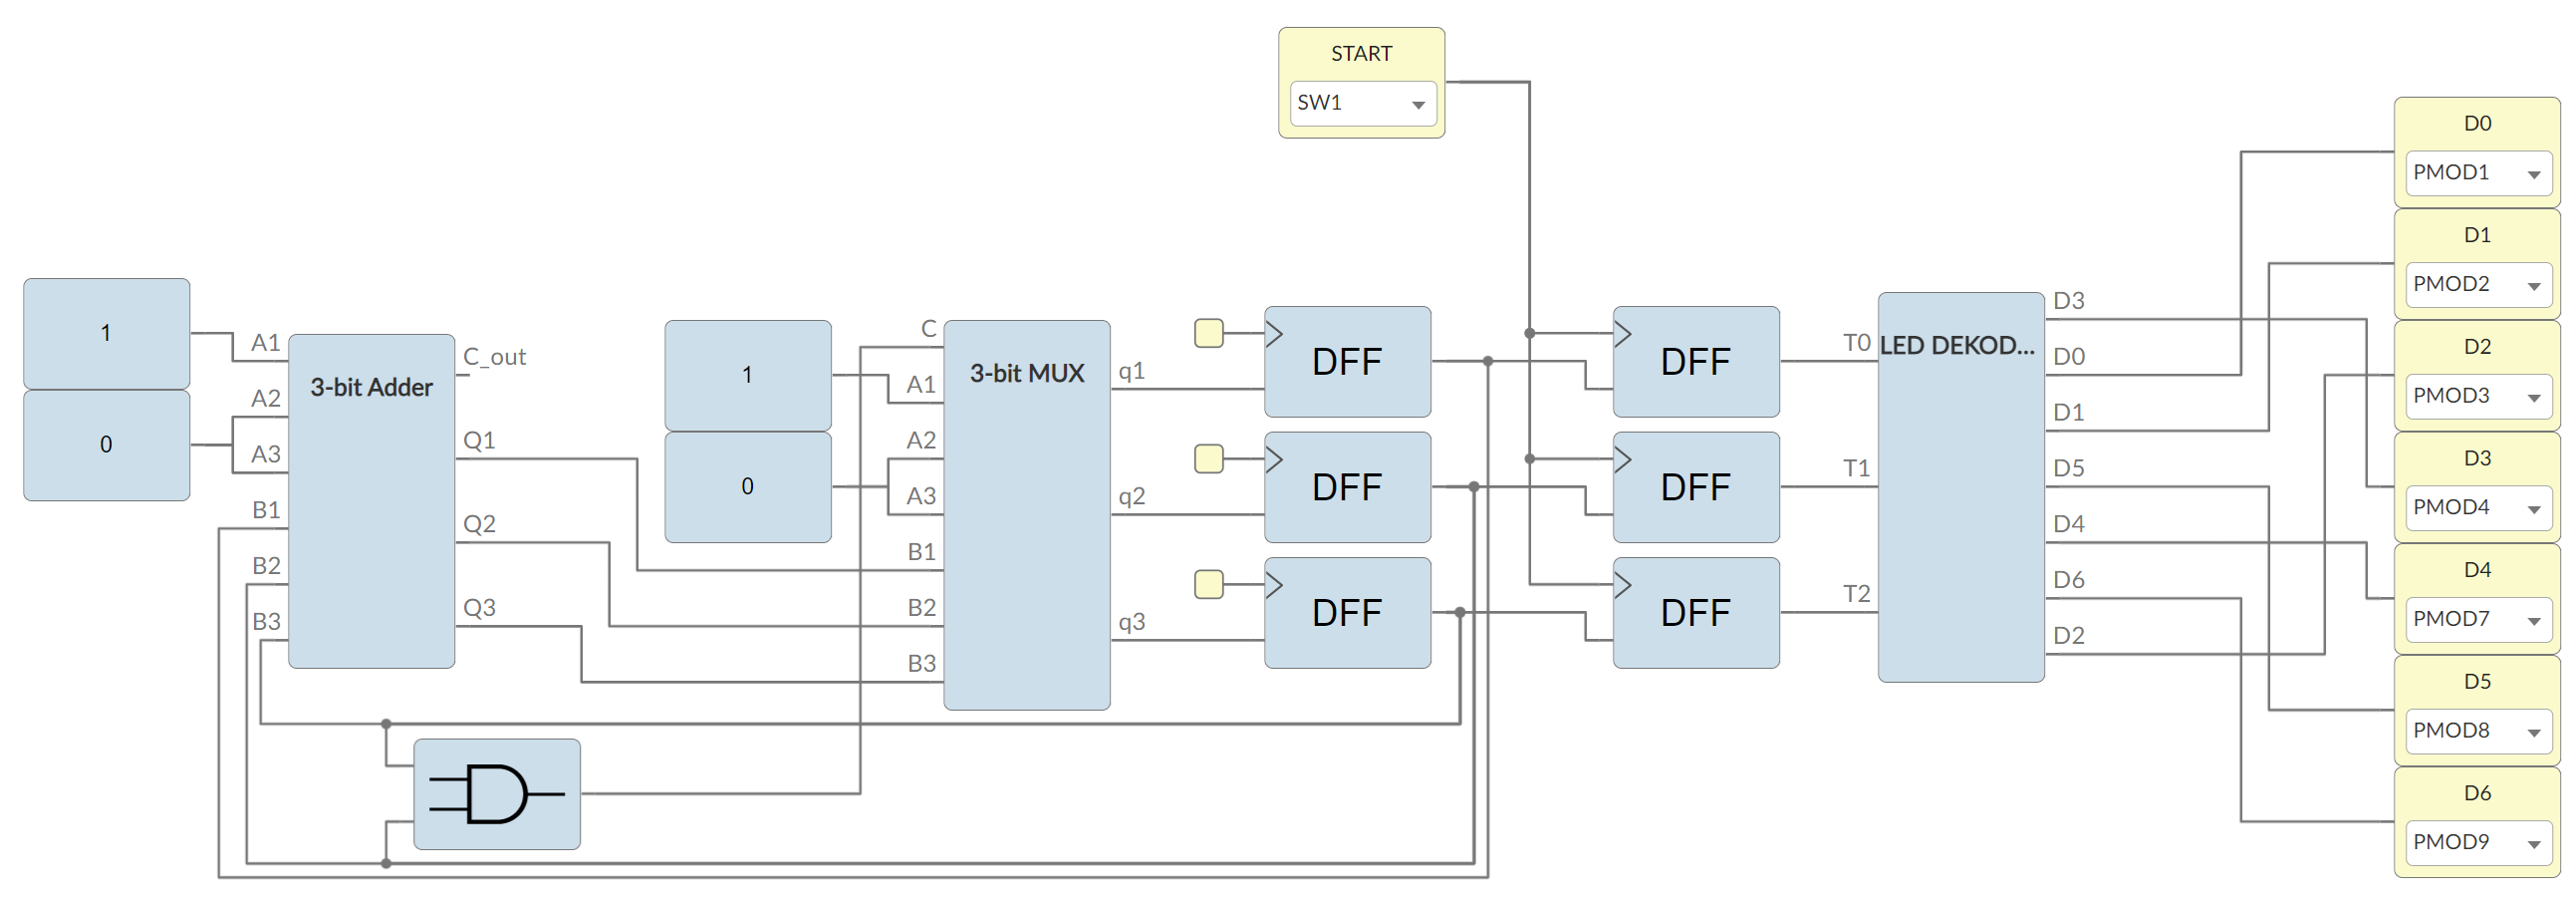
\includegraphics[width=0.9\textwidth]{Bilder/Realisert.png} 
  \caption{Overblikk over den realiserte kretsen}
  \label{fig:Fig2}
\end{figure}


Figur \ref{fig:Fig3} viser realiseringen av en 3-bits fulladderer. Den er realiser med tre XOR porter som legger sammen ingang A og B dersom de er ulike, og sender det til utgang q. Deretter brukes en kombinasjon av AND og OR porter for å sende bæretallet videre. 

\begin{figure}[htbp]
  \centering
  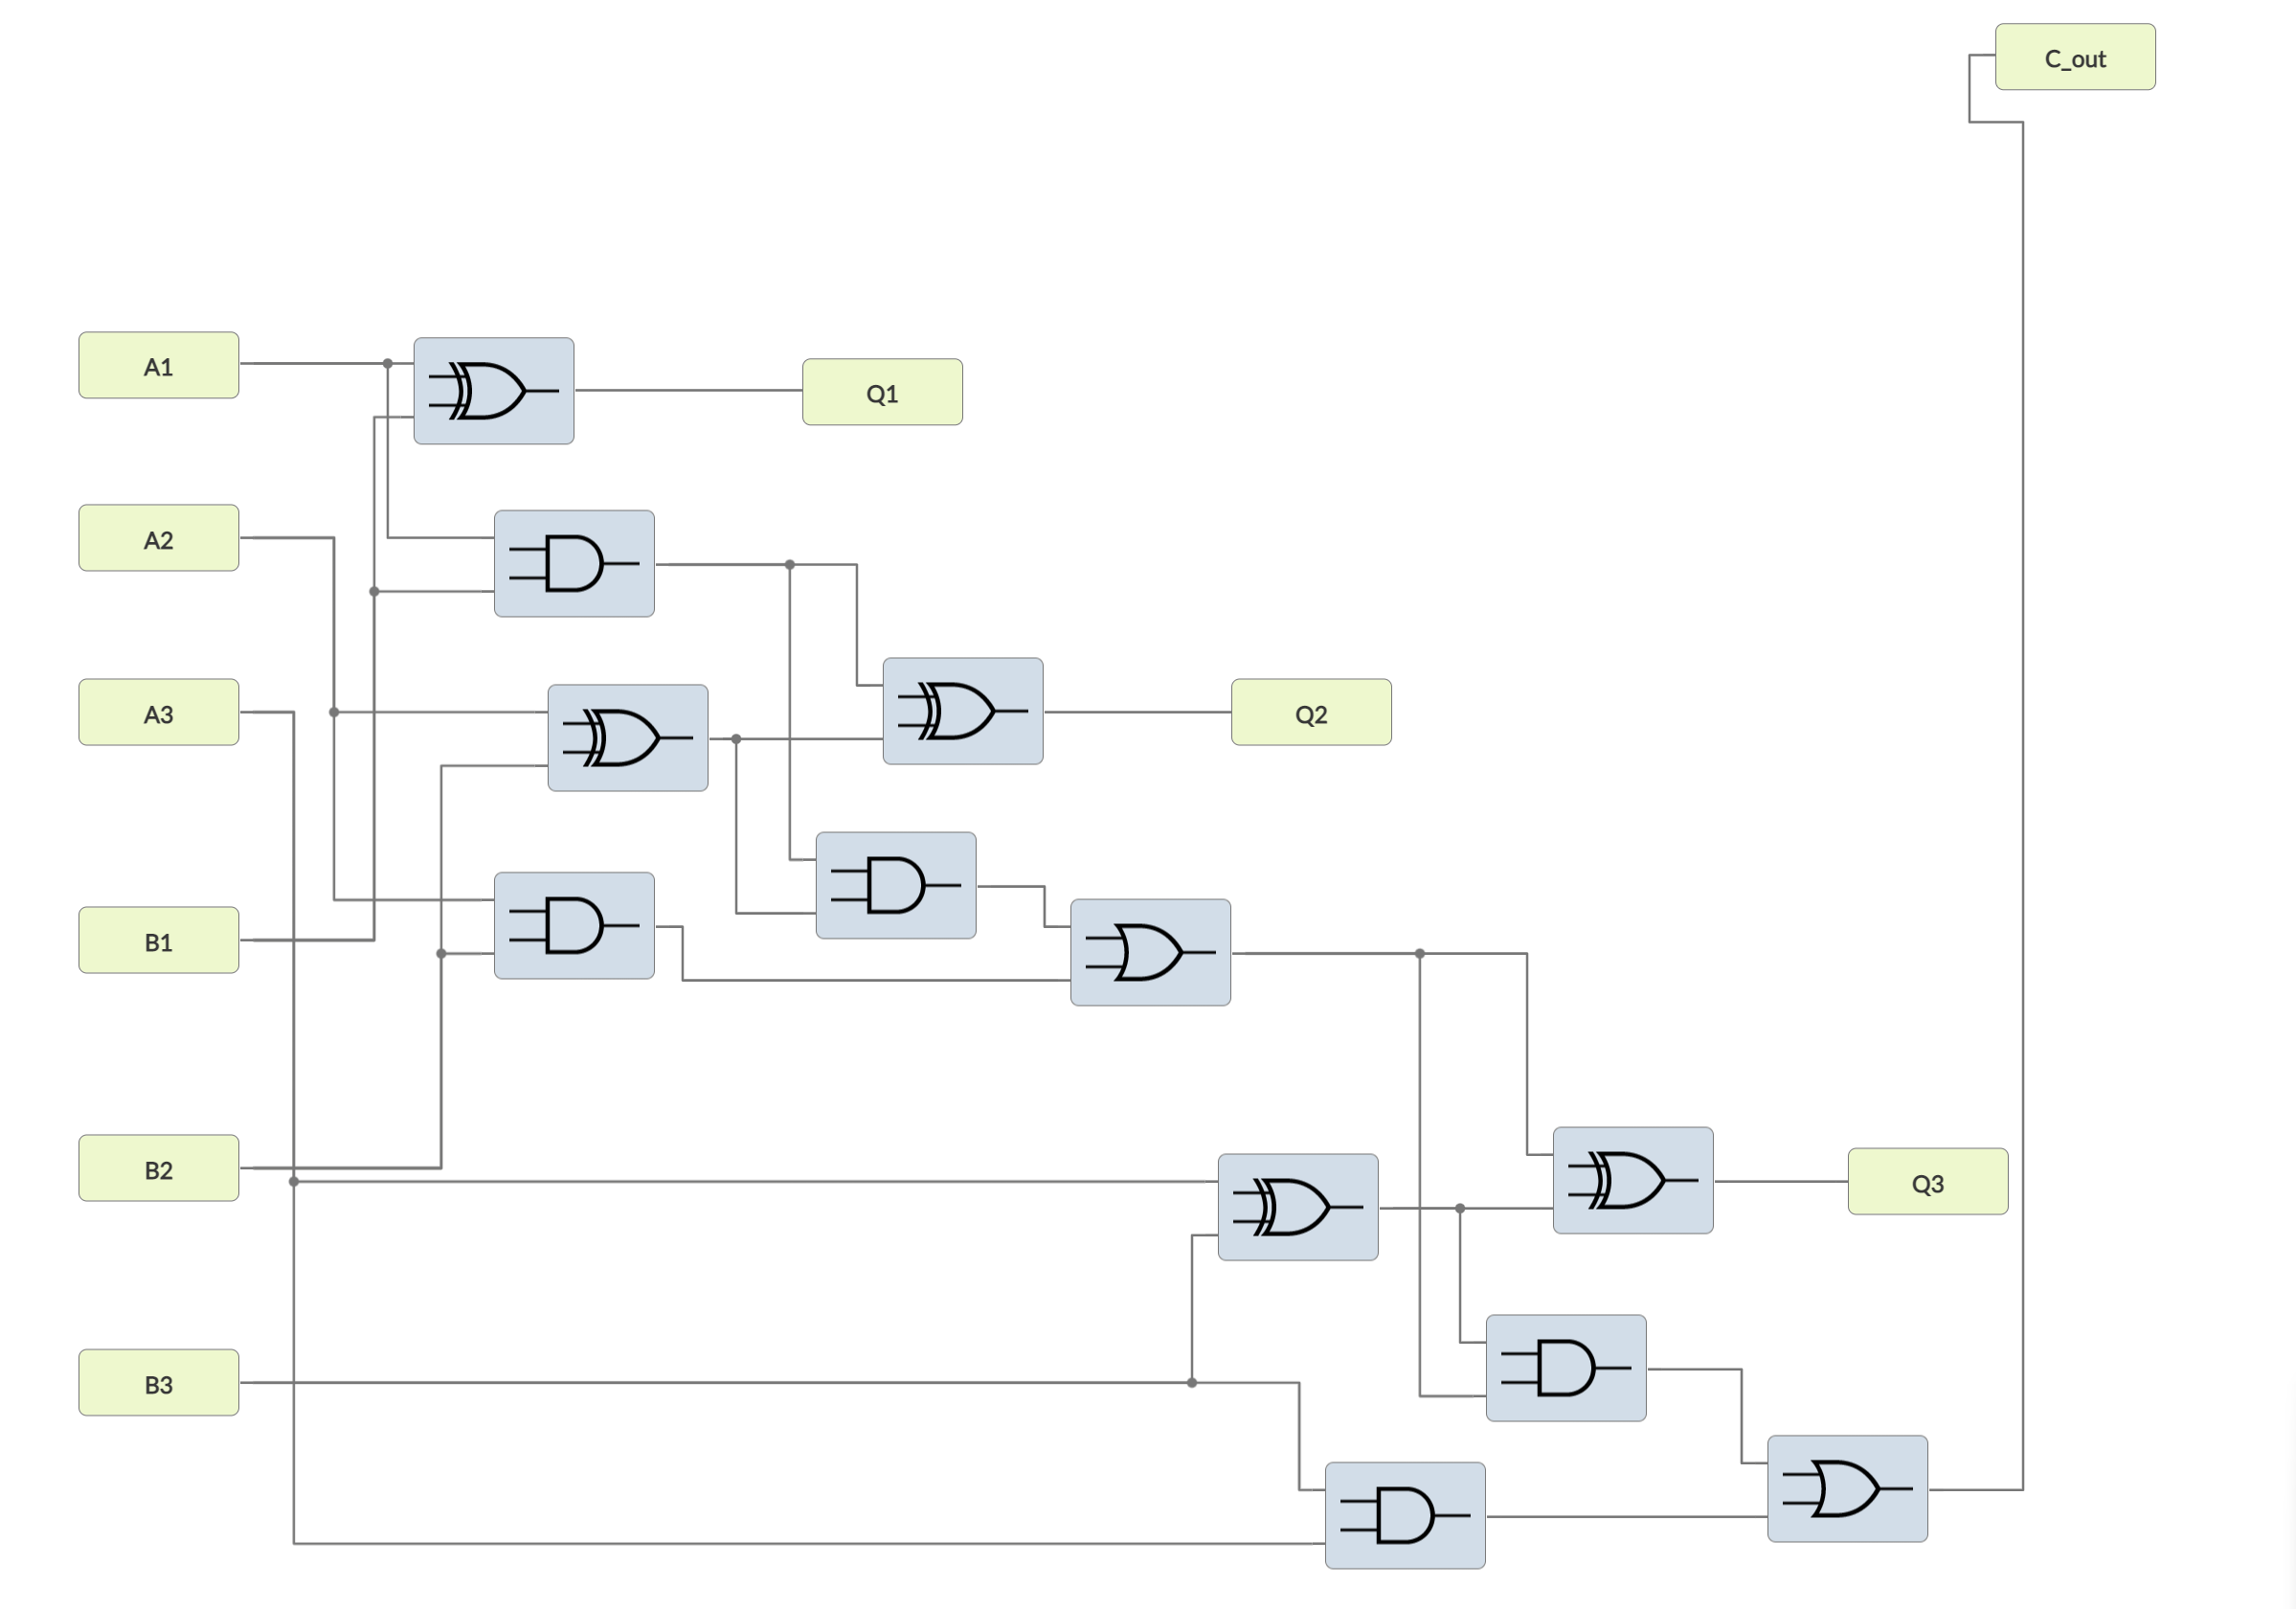
\includegraphics[width=0.6\textwidth]{Bilder/3-bit_adderer.png} 
  \caption{Fulladderer}
  \label{fig:Fig3}
\end{figure}

Figur \ref{fig:Fig4} viser realiseringen av en 3-bits mux, hvor man utnytter FPGAen sine interne MUXer.

\begin{figure}[htbp]
  \centering
  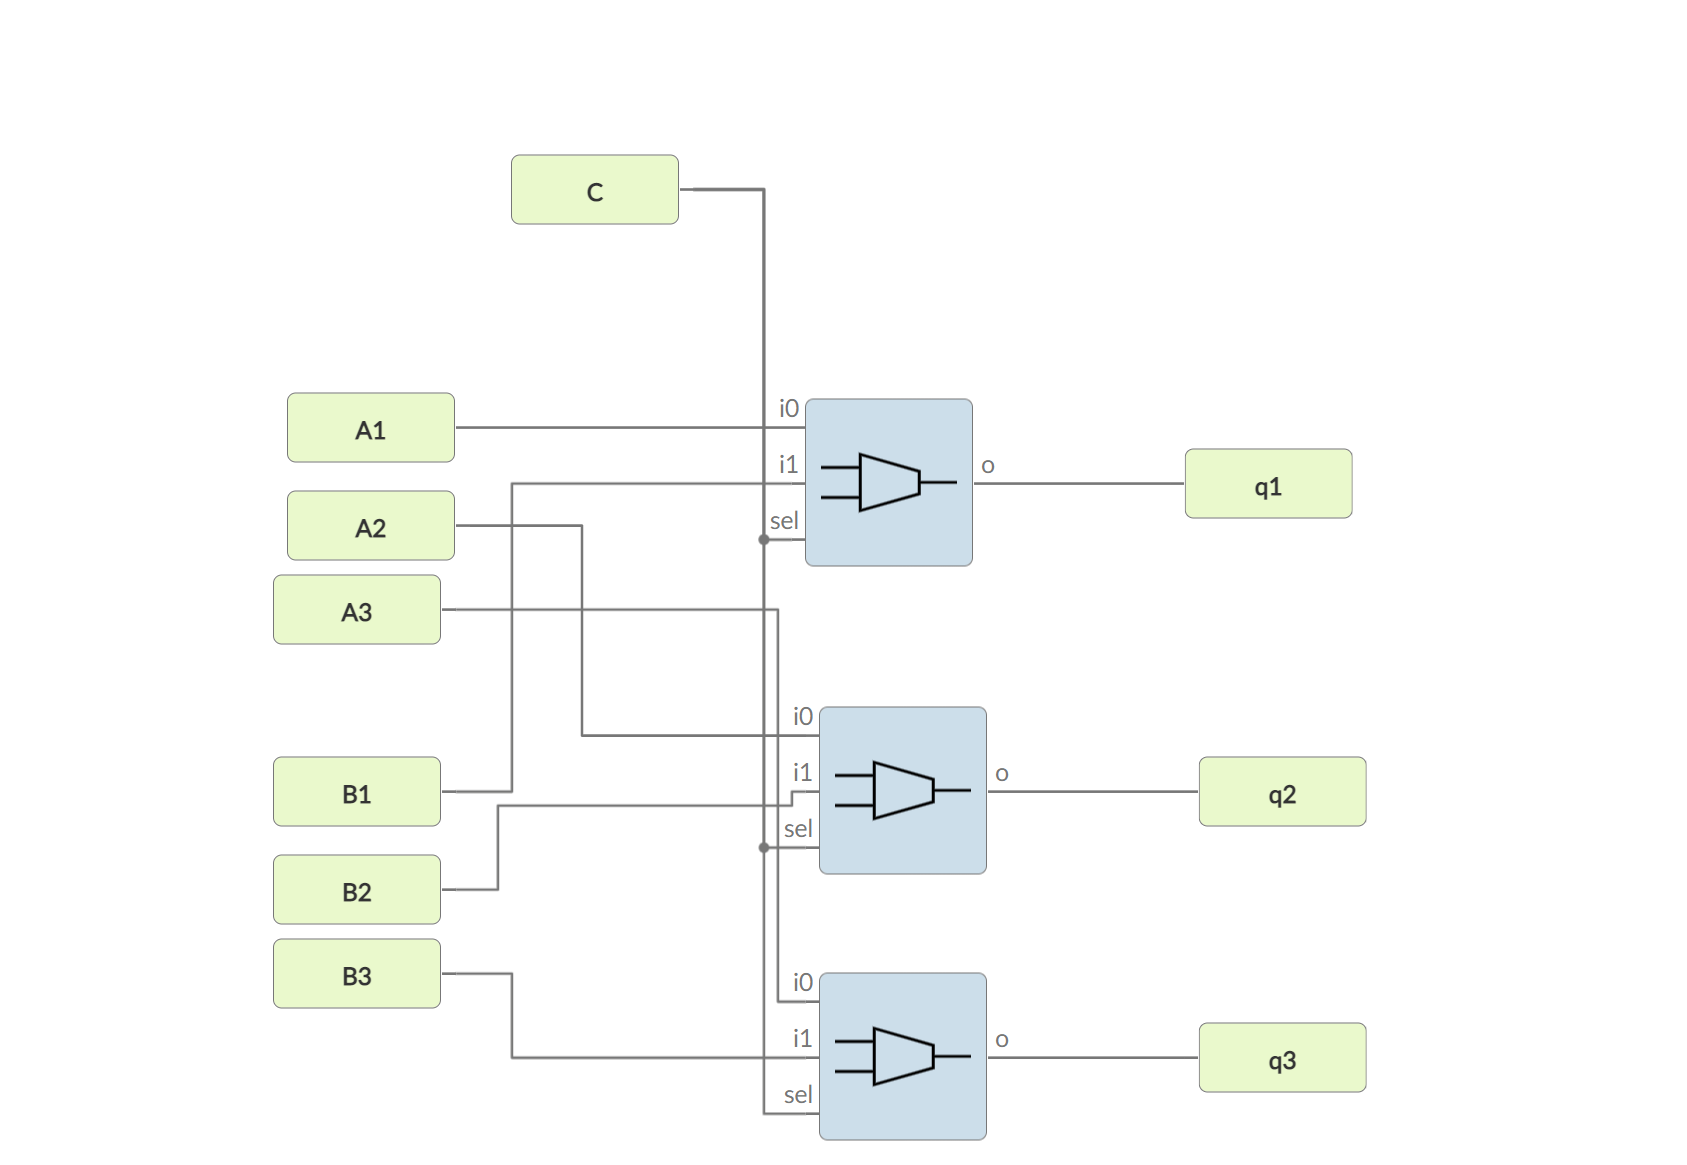
\includegraphics[width=0.6\textwidth]{Bilder/3-bit_MUX.png} 
  \caption{3-bits mux}
  \label{fig:Fig4}
\end{figure}

For at LED lysene skal lyse i et mønster som tilsvarer terningens øyne, må vi ha en dekoder som kan dekode terningkastet til et mønster. I figur \ref{fig:Fig5} viser vi realiseringen av en dekoderen og i tabell \ref{table:tab1} vises sannhetstabellen for dekoderen. Figur \ref{fig:Fig6} viser LED matrisen som er koblet opp til dekoderen med navnene utgangen av dekoderen i riktig mønster.

\begin{figure}[!h]
  \centering
  \begin{minipage}[c]{0.6\textwidth}
    \centering
    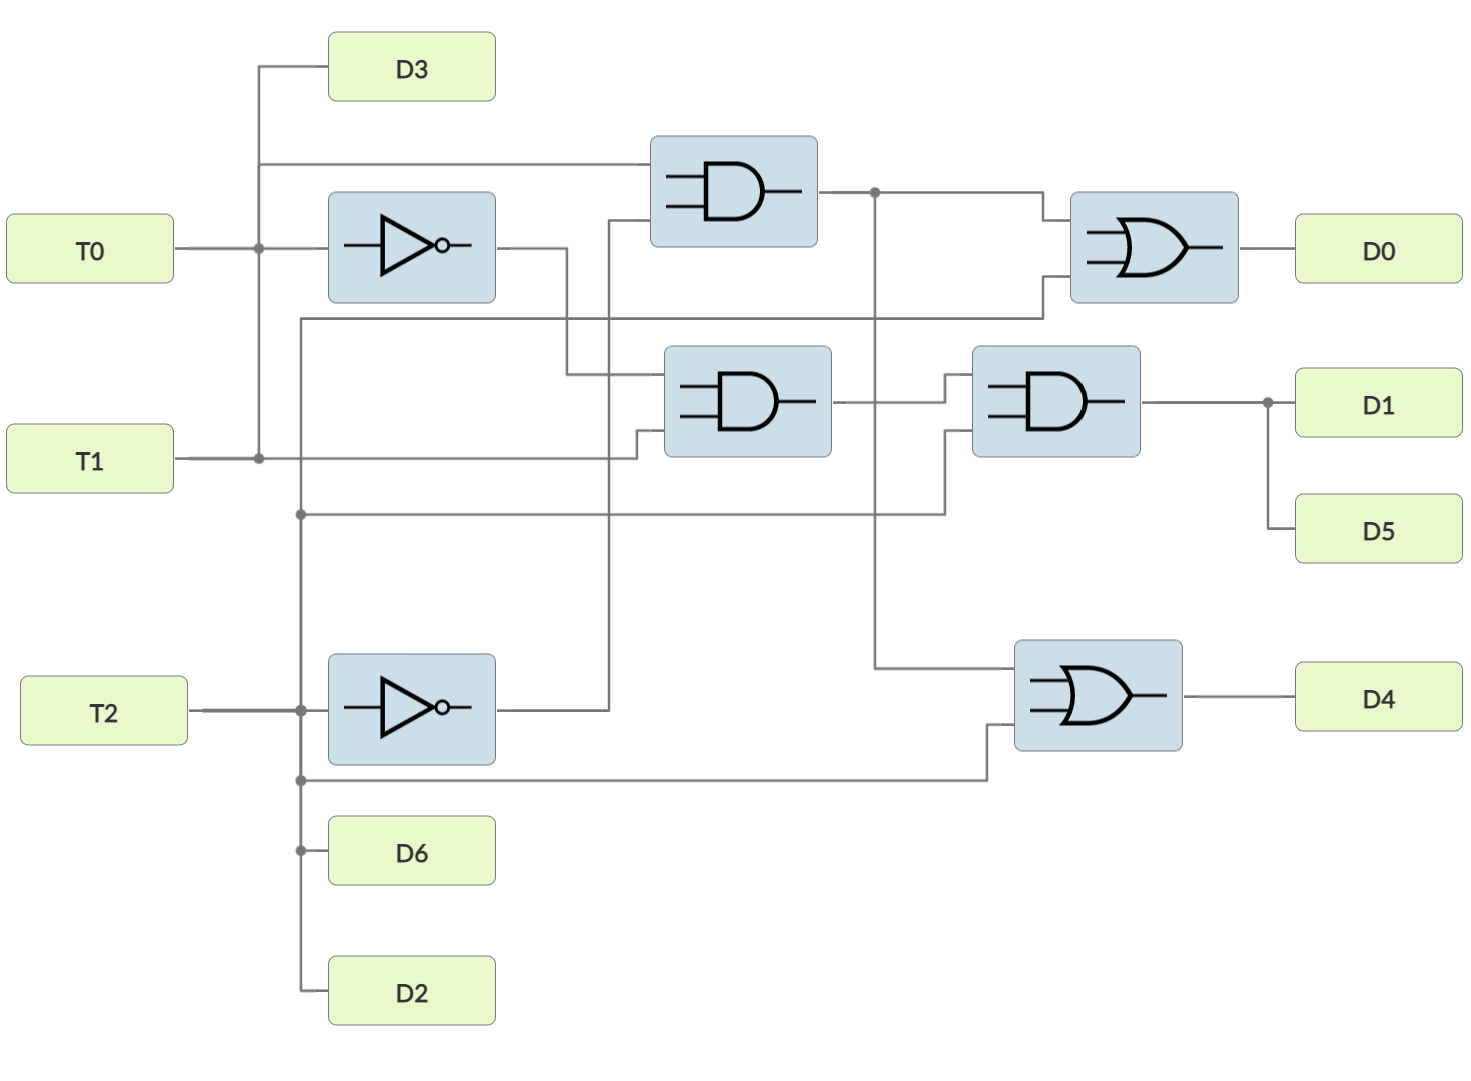
\includegraphics[width=1\textwidth]{Bilder/Dekoder.png} 
    \caption{}
    \label{fig:Fig5}   
  \end{minipage}
  \hfill
  \begin{minipage}[c]{0.3\textwidth}
    \centering
    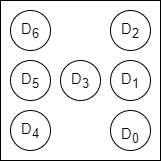
\includegraphics[width=1\textwidth]{Bilder/LED_Matrix.drawio.png} 
    \caption{}
    \label{fig:Fig6}
  \end{minipage}   
\end{figure}

\begin{table}
  \centering
  \caption{Sannhetstabell for dekoderen}
  \newcolumntype{?}{!{\vrule width 2pt}}
  \begin{tabular}[!h]{ |c|c|c?c|c|c|c|c|c|c| } 
      \hline
      $T_2$ & $T_1$ & $T_0$ & $D_6$ & $D_5$ & $D_4$ & $D_3$ & $D_2$ & $D_1$ & $D_0$\\
      \hline
      0 & 0 & 0 & 0 & 0 & 0 & 0 & 0 & 0 & 0 \\ 
      \hline
      0 & 0 & 1 & 0 & 0 & 0 & 1 & 0 & 0 & 0 \\ 
      \hline
      0 & 1 & 0 & 0 & 0 & 1 & 0 & 0 & 0 & 1 \\ 
      \hline 
      0 & 1 & 1 & 0 & 0 & 1 & 1 & 0 & 0 & 1 \\ 
      \hline
      1 & 0 & 0 & 1 & 0 & 1 & 0 & 1 & 0 & 1 \\ 
      \hline
      1 & 0 & 1 & 1 & 0 & 1 & 1 & 1 & 0 & 1 \\ 
      \hline
      1 & 1 & 0 & 1 & 1 & 1 & 0 & 1 & 1 & 1 \\ 
      \hline
     \end{tabular}
    
    \label{table:tab1} 
\end{table}

Telleren er designet på en slik måte at den aldri teller til mer en 6 (110) så man kan se bort ifra når ingagnssignalet er 111. Dette gjør at de boolske utrykkene som er brukt til å designe dekoderen i figur \ref*{fig:Fig5} blir vesentlig mye enklere. De boolske uttrykkene som er brukt for å designe dekoderen er vist i likningene \ref{eq:1} - \ref{eq:5}.

\begin{equation}
  D_0 = \overline{T_0}T_1T_2
  \label{eq:1}
\end{equation}
\begin{equation}
  D_1 = D_5 = T_0T_1T_2
  \label{eq:2}
\end{equation}
\begin{equation}
  D_2 = D_6 = T_2
  \label{eq:3}
\end{equation}
\begin{equation}
  D_3 = T_0
  \label{eq:4}
\end{equation}
\begin{equation}
  D_4 = \overline{T_2}T_1 + T_2
  \label{eq:5}
\end{equation}

For å måle effektforbruket til terningen så måler vi spenningen over hver av de 7 LEDene og regener strømmen gjennom motstandene for å beregne effektforbruket. I tabell \ref{table:tab2} viser vi målingene av spenningen over hver av LEDene.

\begin{table}[!h]
  \centering
  \caption{Målinger av spenningen over hver av LEDene}
  \newcolumntype{?}{!{\vrule width 2pt}}
  \begin{tabular}[!h]{ |c?c|c|c|c|c|c|c| } 
    \hline
    Terningkast & $V_{LED0}$ & $V_{LED1}$ & $V_{LED2}$ & $V_{LED3}$ & $V_{LED4}$ & $V_{LED5}$ & $V_{LED6}$ \\
    \hline
    1 & - & - & - & 3.234 & - & - & - \\
    \hline
    2 & - & - & 3.123 & - & - & - & 3.123 \\
    \hline
    3 & - & - & 3.123 & 3.123 & - & - & 3.123 \\
    \hline
    4 & 3.132 & - & 3.003 & - & 3.003 & - & 3.132 \\
    \hline
    5 & 3.132 & - & 3.003 & 3.003 & 3.003 & - & 3.132 \\
    \hline
    6 & 3.132 & 3.403 & 3.003 & - & 3.003 & 3.004 & 3.132 \\
    \hline
  \end{tabular}
  
  \label{table:tab2}
\end{table}

Vi regner ut strømmen gjennom motstandene ved å bruke formelen \ref{eq:6}.
\begin{equation}
  I = \frac{V}{R}
  \label{eq:6}
\end{equation}

Der $V$ er spenningen over motstanden og $R$ er motstandens verdi. Vi regner ut strømmen gjennom hver av motstandene og regner deretter ut effektforbruket til hver av LEDene ved å bruke formelen \ref{eq:7}.

\begin{equation}
  P_e = V*I
  \label{eq:7}
\end{equation}

For å regne ut effektforbruket til hver av lysdiodene så må vi vite hvor ofte den lyser, i tilleg til strømmen gjennom den. Vi regner ut hvor ofte hver av LEDene lyser ved å se på sansynligheten til hver verdi terningen kan få og om LEDen lyser ved den verdien. Vi regner ut sansynligheten ved å bruke formelen \ref{eq:8}. 

\begin{equation}
  P = \frac{Antall\ gunstige}{Antall\ mulige}
  \label{eq:8}
\end{equation}

I tabell \ref{table:tab3} kan vi lese ut spenningen over hver av LEDene og hvor mye effekt hver diode bruker.

\begin{table}[!h]
  \centering
  \caption{Effektforbruket til hver av LEDene}
  \begin{tabular}[!h]{ |c|c|c|c|c|c|c| }
    \hline
    Farge &  $V_{Diode}$ & $V_{Total}$ & $I(mA)$ & $P_e(mW)$ & $Antall$ & $Plassering$ \\
    \hline
    Rød & 2.2 & 3.3 & 11.14 & 36.76 & 2 & $D_0, D_4$ \\
    \hline
    Grønn & 2.1 & 3.3 & 11.77 & 38.84 & 2 & $D_6, D_2$ \\
    \hline
    Blå & 2.7 & 3.3 & 5.89 & 19.70 & 3 & 3 $D_5, D_3, D_1$\\
    \hline
  \end{tabular}
  \label{table:tab3}
\end{table}

I tabell \ref{table:tab4} kan vi se hvor ofte hver av LEDene lyser og hvor mye effektforbruket til terningen blir, gitt at kastene er uavhengig hverandre og det er like stor sansynelighet for alle utfall. Så kan vi gange effektforbruket med sansynligheten for at LEDen lyser og derfra regne ut det idielle effektforbruket til terningen.



\begin{table}[!h]
  \centering
  \caption{Sansyneligheten til hver av LEDene og effektforbruk over tid}
  \begin{tabular}[!h]{ |c|c|c|c|c| } 
    \hline
    Plassering & antall ganger den lyser & P (sansynelighet) & Farge & $P \cdot P_e$  \\
    \hline
    $D_0$ & 3 & $\frac{3}{6} = 0.5$ & Rød & $0.5 \cdot 36.76 = 18.88$\\
    \hline
    $D_1$ & 1 & $\frac{1}{6} = 0.167$ & Blå & $0.167 \cdot 19.70 = 3.29$\\
    \hline
    $D_2$ & 5 & $\frac{5}{6} = 0.833$ & Grønn & $0.833 \cdot 38.84 = 32.35$\\
    \hline
    $D_3$ & 3 & $\frac{3}{6} = 0.5$ & Blå & $0.5 \cdot 19.70 = 9.85$\\
    \hline
    $D_4$ & 3 & $\frac{3}{6} = 0.5$ & Rød & $0.5 \cdot 36.76 = 18.38$\\
    \hline
    $D_5$ & 1 & $\frac{3}{6} = 0.167$ & Blå & $0.167 \cdot 19.70 = 3.29$\\
    \hline
    $D_6$ & 5 & $\frac{3}{6} = 0.833$ & Grønn & $0.833 \cdot 38.84 = 32.35$\\
    \hline
  \end{tabular}
  
  \label{table:tab4}
\end{table}

Summen av alle effektforbrukene blir da som vi ser i utregning \ref{eq:9}, 118.39mW. Dette er effektforbruket til terningen når den er i bruk over lang tid.
\begin{equation}
  P_{total} = 18.88 + 3.29 + 32.35 + 9.85 + 18.38 + 3.29 + 32.35 = 118.39 mW
  \label{eq:9}
\end{equation}

Skulle terningen vært mer effekteffektiv så måtte man ha plasert de diodene som bruker minst effekt på de plassene som har størst sansynlighet for å lyse. En potensiell realisering av dette er plottet i tabell \ref{table:tab5}.

\begin{table}[!h]
  \centering
  \caption{Sansyneligheten til hver av LEDene og effektforbruk over tid, optimalisert for effektivitet}
  \begin{tabular}[!h]{ |c|c|c|c|c| }
    \hline
    Plassering & antall ganger den lyser & P (sansynelighet) & Farge & $P \cdot P_e $  \\
    \hline
    $D_0$ & 3 & $\frac{3}{6} = 0.5$ & Rød & $0.5 \cdot 36.76 = 18.38$\\
    \hline
    $D_1$ & 1 & $\frac{1}{6} = 0.167$ & Grønn & $0.167 \cdot 38.84 = 6.49$\\
    \hline
    $D_2$ & 5 & $\frac{5}{6} = 0.833$ & Blå & $0.833 \cdot 19.70 = 17.40$\\
    \hline
    $D_3$ & 3 & $\frac{3}{6} = 0.5$ & Blå & $0.5 \cdot 19.70 = 9.85$\\
    \hline
    $D_4$ & 3 & $\frac{3}{6} = 0.5$ & Rød & $0.5 \cdot 36.76 = 18.38$\\
    \hline
    $D_5$ & 1 & $\frac{3}{6} = 0.167$ & Grønn & $0.167 \cdot 38.84 = 6.49$\\
    \hline
    $D_6$ & 5 & $\frac{3}{6} = 0.833$ & Blå & $0.833 \cdot 19.70 = 17.40$\\
    \hline
  \end{tabular}
  \label{table:tab5}
\end{table}

Summen av alle effektforbrukene blir da som vi ser i utregning \ref{eq:10} 79.38mW. Dette er effektforbruket til terningen når den er i bruk over lang tid.

\begin{equation}
  P_{total} = 18.38 + 6.49 + 17.40 + 9.85 + 18.38 + 6.49 + 17.40 = 79.38 mW
  \label{eq:10}
\end{equation}

Besparelsen blir da som vis i utregning \ref{eq:11} 39.01mW. Dette er en besparelse på 33.2\% av det idielle effektforbruket til terningen.

\begin{equation}
  P_{besparelse} = 118.39 - 79.38 = 39.01 mW
  \label{eq:11}
\end{equation}

